% SPDX-FileCopyrightText: 2022 Harish Rajagopal <harish.rajagopals@gmail.com>
%
% SPDX-License-Identifier: GPL-3.0-or-later

\documentclass[10pt, a4paper]{letter}
\usepackage[margin=25mm]{geometry}  % for setting page margins
\usepackage{xcolor}  % for setting colours
\usepackage[pdfusetitle]{hyperref}  % control hyperlink formatting and auto-add PDF metadata
\usepackage{fontawesome5}  % for icons like GitHub, email, mobile, etc.
\usepackage{fontspec}  % for changing the default font
\usepackage{lipsum}  % for filler text in the template
\usepackage{graphicx}  % for photo and handwritten signature
\usepackage{tcolorbox,graphicx}  % for padding the handwritten signature
\usepackage{multirow}  % for aligning the photo within the header

% Use the TeX Gyre Pagella font, similar to Palatino
\setmainfont{TeX Gyre Pagella}

% Define colours
\definecolor{accent}{HTML}{888888}
\definecolor{headings}{HTML}{000000}
\definecolor{text}{HTML}{444444}
\definecolor{misc}{HTML}{888888}
\definecolor{background}{HTML}{ffffff}

% Set global colours
\color{text}
\pagecolor{background}

% Custom command for miscellaneous text
\newcommand{\misc}[1]{\textcolor{misc}{\textit{#1}}}

% Letter setup
\title{R. Harish --- Cover Letter}
\author{Harish Rajagopal}
\signature{\unskip{}Harish Rajagopal}  % remove manual space for handwritten signature
% SPDX-FileCopyrightText: 2022 Harish Rajagopal <harish.rajagopals@gmail.com>
%
% SPDX-License-Identifier: GPL-3.0-or-later

\newcommand{\recipient}{%
    Hiring Manager\\
    Company Name\\
    Address%
}
\newcommand{\salutation}{Sir or Madam}

\date{\misc{\today}}

% Miscellaneous options
\hypersetup{%
    colorlinks=true,  % do not draw boxes around links, color the links themselves
    urlcolor=accent,
    pdfsubject={Cover Letter},
    pdfkeywords={cover letter}
}
\pagenumbering{gobble}  % hide page numbering
\raggedbottom% align text to the top of the page

\begin{document}

\begin{letter}{\misc{\recipient}}

% SPDX-FileCopyrightText: 2022 Harish Rajagopal <harish.rajagopals@gmail.com>
%
% SPDX-License-Identifier: GPL-3.0-or-later

\newcommand{\sep}{$\cdot$}% dot separator
\newcommand{\gmail}{harish.rajagopals@gmail.com}

\begin{flushleft}

\textcolor{headings}{%
\begin{tabular}{l l}
    \multirow{3}{*}[1.5mm]{
\includegraphics[height=17mm]{pic.jpg}\hspace{3mm}}
    & \textsc{\huge Harish Rajagopal} \\[2mm]
    & Computer Science Masters \sep{} ETH Zürich \\[1mm]
    & \faGithub{} \href{https://github.com/rharish101}{rharish101} \sep{}
        \faLinkedin{} \href{https://www.linkedin.com/in/rharish101/}{rharish101} \sep{}
        \faEnvelope{} \href{mailto:\gmail}{\gmail}
\end{tabular}}

\end{flushleft}

\vspace{1cm}
\opening{\textcolor{headings}{\textbf{Dear \salutation,}}}
\lipsum[1]\par
\lipsum[2]\par
\lipsum[3]

\closing{%
    Best regards,\\
    \tcbox[boxrule=-1pt,colback=background,nobeforeafter,boxsep=1mm]{%
        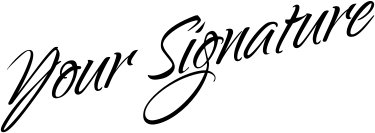
\includegraphics[height=4\baselineskip]{signature.png}%
    }%
}

\end{letter}

\end{document}
